\documentclass{standalone}
\usepackage{tikz}
\usetikzlibrary{patterns}
\usetikzlibrary{positioning}
\usetikzlibrary{patterns, positioning}
\usetikzlibrary{shapes.misc}
\usepackage[outline]{contour}
\contourlength{1.5pt} 
\usepackage[sfdefault]{ClearSans}

\begin{document}
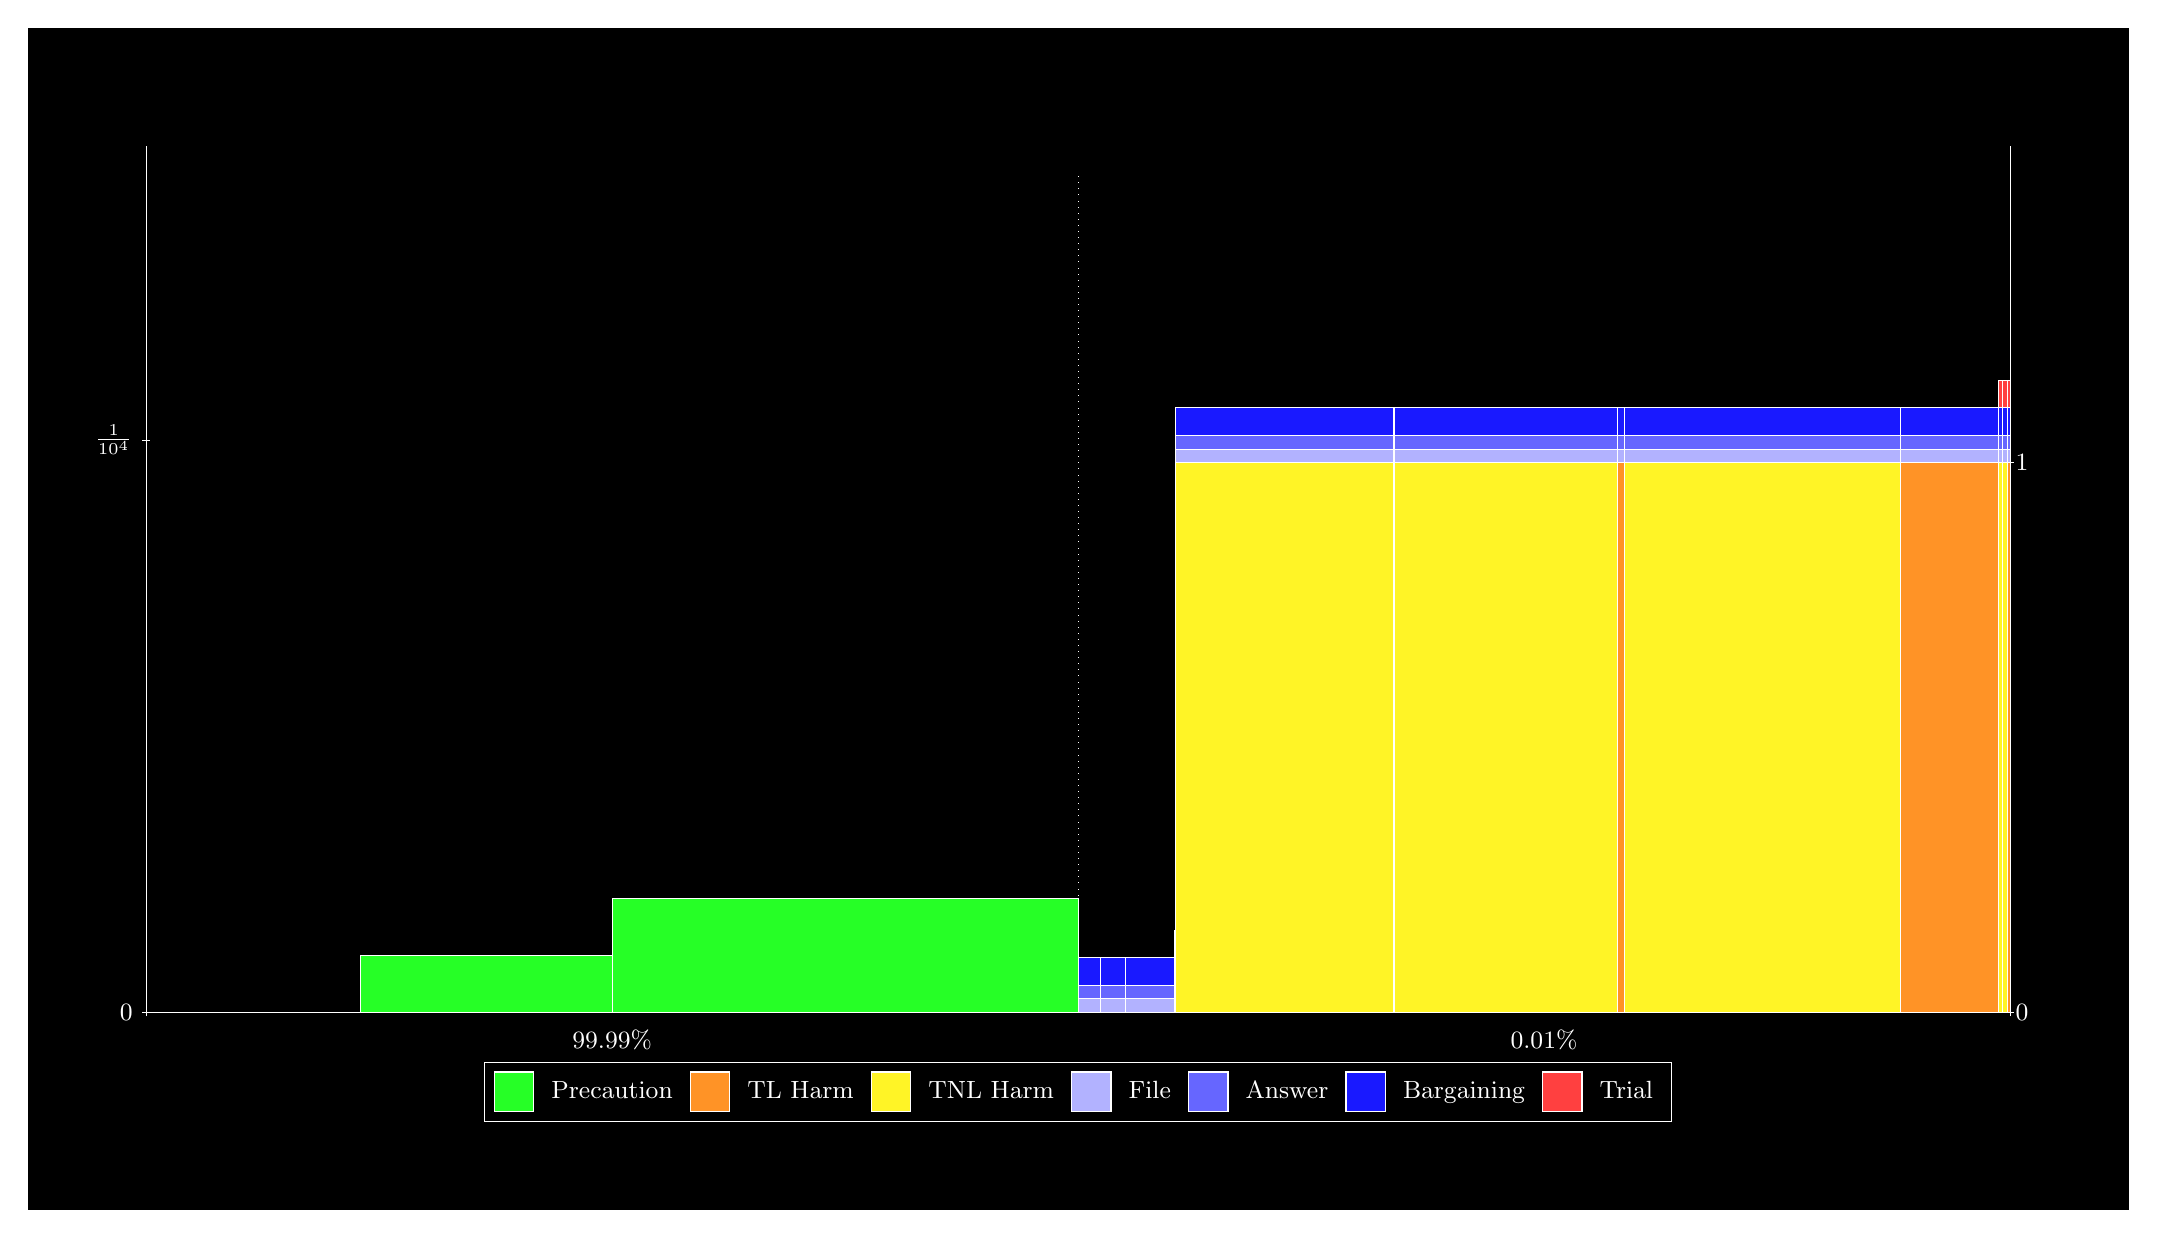
\begin{tikzpicture}
\draw[fill=black] (0,0) rectangle (26.667,15);
\draw[fill=green!85,draw=white,very thin] (4.2218,2.5) rectangle (7.4166,3.2272);
\draw[fill=green!85,draw=white,very thin] (7.4166,2.5) rectangle (13.333,3.9544);
\draw[fill=blue!30,draw=white,very thin] (13.333,2.5) rectangle (13.612,2.6746);
\draw[fill=blue!60,draw=white,very thin] (13.333,2.6746) rectangle (13.612,2.8491);
\draw[fill=blue!90,draw=white,very thin] (13.333,2.8491) rectangle (13.612,3.1983);
\draw[fill=green!85,draw=white,very thin] (13.612,2.5) rectangle (13.934,2.5001);
\draw[fill=blue!30,draw=white,very thin] (13.612,2.5001) rectangle (13.934,2.6746);
\draw[fill=blue!60,draw=white,very thin] (13.612,2.6746) rectangle (13.934,2.8492);
\draw[fill=blue!90,draw=white,very thin] (13.612,2.8492) rectangle (13.934,3.1983);
\draw[fill=green!85,draw=white,very thin] (13.934,2.5) rectangle (14.55,2.5001);
\draw[fill=blue!30,draw=white,very thin] (13.934,2.5001) rectangle (14.55,2.6747);
\draw[fill=blue!60,draw=white,very thin] (13.934,2.6747) rectangle (14.55,2.8493);
\draw[fill=blue!90,draw=white,very thin] (13.934,2.8493) rectangle (14.55,3.1984);
\draw[fill=green!85,draw=white,very thin] (14.55,2.5) rectangle (14.561,2.5001);
\draw[fill=blue!30,draw=white,very thin] (14.55,2.5001) rectangle (14.561,2.6746);
\draw[fill=blue!60,draw=white,very thin] (14.55,2.6746) rectangle (14.561,2.8492);
\draw[fill=blue!90,draw=white,very thin] (14.55,2.8492) rectangle (14.561,3.1983);
\draw[fill=red!75,draw=white,very thin] (14.55,3.1983) rectangle (14.561,3.5475);
\draw[fill=yellow!85,draw=white,very thin] (14.561,2.5) rectangle (17.331,9.4826);
\draw[fill=blue!30,draw=white,very thin] (14.561,9.4826) rectangle (17.331,9.6572);
\draw[fill=blue!60,draw=white,very thin] (14.561,9.6572) rectangle (17.331,9.8317);
\draw[fill=blue!90,draw=white,very thin] (14.561,9.8317) rectangle (17.331,10.181);
\draw[fill=orange!85,draw=white,very thin] (17.331,2.5) rectangle (17.345,9.4826);
\draw[fill=blue!30,draw=white,very thin] (17.331,9.4826) rectangle (17.345,9.6572);
\draw[fill=blue!60,draw=white,very thin] (17.331,9.6572) rectangle (17.345,9.8317);
\draw[fill=blue!90,draw=white,very thin] (17.331,9.8317) rectangle (17.345,10.181);
\draw[fill=green!85,draw=white,very thin] (17.345,2.5) rectangle (20.184,2.5001);
\draw[fill=yellow!85,draw=white,very thin] (17.345,2.5001) rectangle (20.184,9.4827);
\draw[fill=blue!30,draw=white,very thin] (17.345,9.4827) rectangle (20.184,9.6572);
\draw[fill=blue!60,draw=white,very thin] (17.345,9.6572) rectangle (20.184,9.8318);
\draw[fill=blue!90,draw=white,very thin] (17.345,9.8318) rectangle (20.184,10.181);
\draw[fill=green!85,draw=white,very thin] (20.184,2.5) rectangle (20.275,2.5001);
\draw[fill=orange!85,draw=white,very thin] (20.184,2.5001) rectangle (20.275,9.4827);
\draw[fill=blue!30,draw=white,very thin] (20.184,9.4827) rectangle (20.275,9.6572);
\draw[fill=blue!60,draw=white,very thin] (20.184,9.6572) rectangle (20.275,9.8318);
\draw[fill=blue!90,draw=white,very thin] (20.184,9.8318) rectangle (20.275,10.181);
\draw[fill=green!85,draw=white,very thin] (20.275,2.5) rectangle (23.781,2.5001);
\draw[fill=yellow!85,draw=white,very thin] (20.275,2.5001) rectangle (23.781,9.4827);
\draw[fill=blue!30,draw=white,very thin] (20.275,9.4827) rectangle (23.781,9.6573);
\draw[fill=blue!60,draw=white,very thin] (20.275,9.6573) rectangle (23.781,9.8319);
\draw[fill=blue!90,draw=white,very thin] (20.275,9.8319) rectangle (23.781,10.181);
\draw[fill=green!85,draw=white,very thin] (23.781,2.5) rectangle (25.024,2.5001);
\draw[fill=orange!85,draw=white,very thin] (23.781,2.5001) rectangle (25.024,9.4827);
\draw[fill=blue!30,draw=white,very thin] (23.781,9.4827) rectangle (25.024,9.6573);
\draw[fill=blue!60,draw=white,very thin] (23.781,9.6573) rectangle (25.024,9.8319);
\draw[fill=blue!90,draw=white,very thin] (23.781,9.8319) rectangle (25.024,10.181);
\draw[fill=yellow!85,draw=white,very thin] (25.024,2.5) rectangle (25.064,9.4826);
\draw[fill=blue!30,draw=white,very thin] (25.024,9.4826) rectangle (25.064,9.6572);
\draw[fill=blue!60,draw=white,very thin] (25.024,9.6572) rectangle (25.064,9.8317);
\draw[fill=blue!90,draw=white,very thin] (25.024,9.8317) rectangle (25.064,10.181);
\draw[fill=red!75,draw=white,very thin] (25.024,10.181) rectangle (25.064,10.53);
\draw[fill=orange!85,draw=white,very thin] (25.064,2.5) rectangle (25.074,9.4826);
\draw[fill=blue!30,draw=white,very thin] (25.064,9.4826) rectangle (25.074,9.6572);
\draw[fill=blue!60,draw=white,very thin] (25.064,9.6572) rectangle (25.074,9.8317);
\draw[fill=blue!90,draw=white,very thin] (25.064,9.8317) rectangle (25.074,10.181);
\draw[fill=red!75,draw=white,very thin] (25.064,10.181) rectangle (25.074,10.53);
\draw[fill=green!85,draw=white,very thin] (25.074,2.5) rectangle (25.129,2.5001);
\draw[fill=yellow!85,draw=white,very thin] (25.074,2.5001) rectangle (25.129,9.4827);
\draw[fill=blue!30,draw=white,very thin] (25.074,9.4827) rectangle (25.129,9.6572);
\draw[fill=blue!60,draw=white,very thin] (25.074,9.6572) rectangle (25.129,9.8318);
\draw[fill=blue!90,draw=white,very thin] (25.074,9.8318) rectangle (25.129,10.181);
\draw[fill=red!75,draw=white,very thin] (25.074,10.181) rectangle (25.129,10.53);
\draw[fill=green!85,draw=white,very thin] (25.129,2.5) rectangle (25.167,2.5001);
\draw[fill=orange!85,draw=white,very thin] (25.129,2.5001) rectangle (25.167,9.4827);
\draw[fill=blue!30,draw=white,very thin] (25.129,9.4827) rectangle (25.167,9.6572);
\draw[fill=blue!60,draw=white,very thin] (25.129,9.6572) rectangle (25.167,9.8318);
\draw[fill=blue!90,draw=white,very thin] (25.129,9.8318) rectangle (25.167,10.181);
\draw[fill=red!75,draw=white,very thin] (25.129,10.181) rectangle (25.167,10.53);
\draw[white,very thin] (1.5,2.5) -- (1.5,13.5);
\draw[white,very thin] (1.45,2.5) -- (1.55,2.5);
\node[font=\small,text=white, anchor=east] at (1.45, 2.5) {0};
\draw[white,very thin] (1.45,9.7721) -- (1.55,9.7721);
\node[font=\small,text=white, anchor=east] at (1.45, 9.7721) {$\frac{1}{10^{4}}$};

\draw[white,dotted,very thin] (13.333,2.83) -- (13.333,13.17);
\draw[white,very thin] (25.167,2.5) -- (25.167,13.5);
\draw[white,very thin] (25.117,2.5) -- (25.217,2.5);
\node[font=\small,text=white, anchor=west] at (25.117, 2.5) {0};
\draw[white,very thin] (25.117,9.4826) -- (25.217,9.4826);
\node[font=\small,text=white, anchor=west] at (25.117, 9.4826) {1};

\draw[white,very thin] (1.5,2.5) -- (25.167,2.5);
\draw[white,very thin] (1.5,2.45) -- (1.5,2.55);
\node[font=\small,text=white, anchor=north] at (1.5, 2.45) {};
\draw[white,very thin] (25.167,2.45) -- (25.167,2.55);
\node[font=\small,text=white, anchor=north] at (25.167, 2.45) {};

\node[font=\small,text=white,anchor=south] at (7.4167, 1.9) {99.99\%};
\node[font=\small,text=white,anchor=south] at (19.25, 1.9) {0.01\%};
\draw (13.3333,2.5) node (B) {};
\begin{scope}[align=center]
\matrix[scale=0.5,draw=white,below=0.5cm of B,nodes={draw},column sep=0.1cm]{
\node[rectangle,draw,minimum width=0.5cm,minimum height=0.5cm,fill=green!85]{}; & \node[draw=none,font=\small,text=white]{Precaution}; &
\node[rectangle,draw,minimum width=0.5cm,minimum height=0.5cm,fill=orange!85]{}; & \node[draw=none,font=\small,text=white]{TL Harm}; &
\node[rectangle,draw,minimum width=0.5cm,minimum height=0.5cm,fill=yellow!85]{}; & \node[draw=none,font=\small,text=white]{TNL Harm}; &
\node[rectangle,draw,minimum width=0.5cm,minimum height=0.5cm,fill=blue!30]{}; & \node[draw=none,font=\small,text=white]{File}; &
\node[rectangle,draw,minimum width=0.5cm,minimum height=0.5cm,fill=blue!60]{}; & \node[draw=none,font=\small,text=white]{Answer}; &
\node[rectangle,draw,minimum width=0.5cm,minimum height=0.5cm,fill=blue!90]{}; & \node[draw=none,font=\small,text=white]{Bargaining}; &
\node[rectangle,draw,minimum width=0.5cm,minimum height=0.5cm,fill=red!75]{}; & \node[draw=none,font=\small,text=white]{Trial}; \\\\
};\end{scope}

\end{tikzpicture}
\end{document}